\documentclass[11pt, a4paper]{article}

\usepackage[margin=1in]{geometry} % manage page dimentions
\usepackage[utf8]{inputenc} % utf-8 encoding
\usepackage[italian]{babel} % italian default text
\usepackage[hidelinks]{hyperref} % link references
\usepackage{bookmark} % 
\usepackage{import} % import other .tex files
\usepackage{amsmath} % math commands
\usepackage{amssymb} % math symbols
\usepackage{amsthm} % math environments
\usepackage{amsmath} % equation align
\usepackage{siunitx} % SI unit
\usepackage{booktabs} % tabular enhance
\usepackage{multirow} % dinamic tabular cell dimentions
\usepackage{longtable} % multi-page table
\usepackage[labelfont=bf, skip=.5em, font=small]{caption} % beautiful caption
\usepackage{subcaption} % subfigure
\usepackage{graphicx} % import graphics
\usepackage{fancyhdr} % custom page header and footer

\graphicspath{{../assets/}} % base graphics path

\setlength{\parskip}{1em} % distance between paragraphs
\setlength{\parindent}{0em} % indentation at beginning of paragraph
\setlength{\headheight}{13.59999pt}

\numberwithin{equation}{section} % equation tag relative to section

\pagestyle{fancy}
\fancyhead[L]{\nouppercase{\leftmark}}
\fancyhead[R]{\textbf{Pag. \thepage}}
\fancyfoot{}

\title{Esperienza 3}
\date{09/12/2021}
\author{}

\begin{document}

\maketitle

\thispagestyle{empty}

\tableofcontents

\section{Obiettivo dell'esperienza}

Lo scopo dell'esperienza è quello di calcolare il valore della resistenza e della capacità di un circuito RC. Per farlo si analizza come varia la differenza di potenziale ai capi di R (\autoref{fig:circuito R}) e/o ai capi di C (\autoref{fig:circuito C}) quando si sottoposto il circuito ad una tensione variabile.

\begin{figure}[ht!]
    \centering
    \begin{subfigure}[c]{.3\textwidth}
        % \import{../assets/}{circuito_osc_R.pdf_tex}
        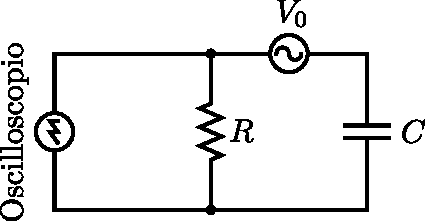
\includegraphics[width=\textwidth]{circuito_osc_R.pdf}
        \caption{Misure ai capi di R}
        \label{fig:circuito R}
    \end{subfigure}
    \hspace{1in}
    \begin{subfigure}[c]{.3\textwidth}
        % \import{../assets/}{circuito_osc_C.pdf_tex}
        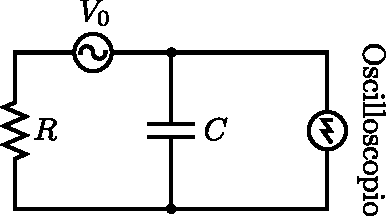
\includegraphics[width=\textwidth]{circuito_osc_C.pdf}
        \caption{Misure ai capi di C}
        \label{fig:circuito C}
    \end{subfigure}
    \caption{Schema circuito}
  \end{figure}

\section{Strumenti e materiali}

\begin{itemize}
    \item Generatore di tensione AC
    \item Multimetro digitale (utilizzato come ohmetro)
    \item Oscilloscopio
    \item Cavi
    \item Breadboard
    \item Resistore
    \item Condensatore
\end{itemize}

\section{Onda quadra}

La prima parte dell'esperimento consiste nell'applicare ai capi del circuito una tensione variabile secondo un'onda quadra di ampiezza \(V_{0}\). La frequenza dell'onda è stata scelta in modo da permettere al condensatore di completare il regime transitorio, passando da una tensione \(V_{0}/2\) fino ad una tensione \(- V_{0}/2\). La curva osservata nell'oscilloscopio rappresenta la tensione \(V_{C}\) ai capi del condensatore in funzione del tempo \(t\) e segue l'\autoref{eq:regime transitorio onda quadra}.

\begin{equation} \label{eq:regime transitorio onda quadra}
    V_{C} = V_{0} \cdot e^{-t/RC} - V_{0}/2
\end{equation}

Per prendere le misure il sistema di riferimento è stato traslato in modo da porre come zero delle ordinate il valore \(- V_{0}/2\) e ottenere l'\autoref{eq:regime transitorio condensatore}.

\begin{equation} \label{eq:regime transitorio condensatore}
    V = V_{0} \cdot e^{-t/RC}
\end{equation}

Noto il valore di \(R = (1.874 \pm 0.004) \; \unit{k\Omega}\) (misurato con il multimetro) si vuole ottenere il valore di \(C\).

\subsection{Dati ed errori}

Sull'oscilloscopio è stato fissato il primo cursore in corrispondenza dell'asintoto della curva a \(- V_{0}/2\); questo sarà lo zero delle ordinate. \\
Il secondo cursore è stato fatto variare in modo da ottenere la differenza di potenziale al variare del tempo. Le misure ottenute sono riportate, insieme ai loro errori già arrotondati, nella \autoref{tab:misure onda quadra}.

\begin{table}[ht!]
    \centering
    \caption{Misure dell'onda quadra}
    \import{../tables/}{onda_quadra_Vt.tex}
    \label{tab:misure onda quadra}
\end{table}

\subsection{Analisi dati}

\begin{equation*}
    V = V_{0} \cdot e^{-t/RC} \implies \ln(V) = \ln(V_{0} \cdot e^{-t/RC}) = \ln(V_{0}) - \frac{t}{RC}
\end{equation*}

Riportando le misure in un grafico semi-logaritmico (come in \autoref{fig:onda quadra pendenze}), ci si aspetta di ottenere una funzione lineare:

\begin{figure}[ht!]
    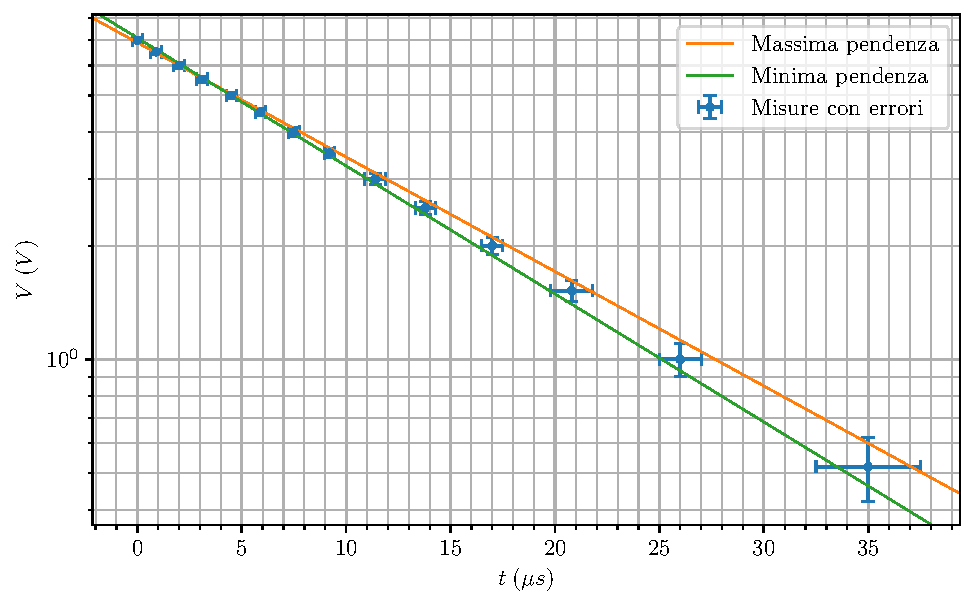
\includegraphics{onda_quadra_V(t)_pendenze.pdf}
    \caption{Grafico semi-logaritmico delle misure dell'onda quadra}
    \label{fig:onda quadra pendenze}
\end{figure}

La retta di massima pendenza passa per i punti \((-0.2, 7)\) e \((35, 0.6)\), mentre la retta di minima pendenza passa per i punti \((0.2, 7)\) e \((34, 0.5)\).

\begin{equation*}
    m_{max} = \frac{\ln(7/0.6)}{- 0.2 - 35} = - 0.06979
    \qquad
    m_{min} = \frac{\ln(7/0.5)}{0.2 - 34} = - 0.07808
\end{equation*}

\begin{align*}
    m_{best} &= \frac{m_{max} + m_{min}}{2} = - 0.0739 \approx - 0.074 \\
    \delta m &= \frac{m_{max} - m_{min}}{2} = 0.0041 \approx 0.004
\end{align*}

\begin{equation}
    m = - 0.074 \pm 0.004
\end{equation}

\newpage

Essendo \(m = \dfrac{1}{RC}\) e conoscendo il valore di \(R = (1.874 \pm 0.004) \; \unit{k\Omega}\).

\begin{align*}
    \varepsilon_R &= \frac{0.004}{1.874} = 0.0021 \approx 0.002 \\
    \varepsilon_m &= \frac{0.004}{0.074} = 0.054 \approx 0.05 \\
    \varepsilon_C &= \sqrt{\varepsilon_R^{2} + \varepsilon_m^{2}} = 0.050 % review
\end{align*}

\begin{equation}
    C = \frac{R}{m} = 25.32 \pm 1.27 \approx (25.3 \pm 1.3) \; \unit{nF}
\end{equation}

\section{Onda sinusoidale}

La seconda parte dell'esperimento consiste nel sottoporre il circuito a un regime di tensione sinusoidale, variando la frequenza in entrata; abbiamo poi misurato la tensione in uscita del circuito ai capi di $C$ e ai capi di $R$, così come il tempo di risposta del circuito. Con questi dati abbiamo determinato il modulo della \emph{funzione di trasferimento} $|A_{C}|$, la sua fase $\phi$ e la frequenza di taglio $f_{0}$.

% todo
% 
%    Tensione R
%      - Ampiezza
%      - Fase
%    Tensione C
%      - (...)

\subsection{Funzione di trasferimento ai capi di $C$}

\subsubsection{Dati ed errori}

Nella \autoref{tab:misure onda sinusoidale C} sono riportati i risultati delle misurazioni effettuate con i relativi errori

\begin{table}[ht!]
    \centering
    \caption{Misure dell'onda sinusoidale ai capi di $C$}
    \import{../tables/}{onda_sin_VC.tex}
    \label{tab:misure onda sinusoidale C}
\end{table}

\newpage

\subsubsection{Analisi dati}

Con i dati raccolti si calcola il modulo della funzione di trasferimento $|A_{C}|$ al variare della frequenza utilizzando l'\autoref{eq:funzione di trasferimento C}

\begin{align} \label{eq:funzione di trasferimento C}
    \begin{split}
        |A_{C}| &= \frac{V_{out}}{V_{in}} \\
        \varepsilon_{|A_{C}|} &= \frac{\delta V_{out}}{V_{out}} + \frac{\delta V_{in}}{V_{in}}
    \end{split}
\end{align}

\begin{table}[ht!]
    \centering
    \caption{Valori di $|A_{C}|$}
    \import{../tables/}{onda_sin_AC.tex}
    \label{tab:funzione di trasferimento C}
\end{table}

Riportando le misure della \autoref{tab:funzione di trasferimento C} in un grafico logaritmico $|A_{C}|(f)$ si ottiene la \autoref{fig:funzione di trasferimento C}

\begin{figure}[ht!]
    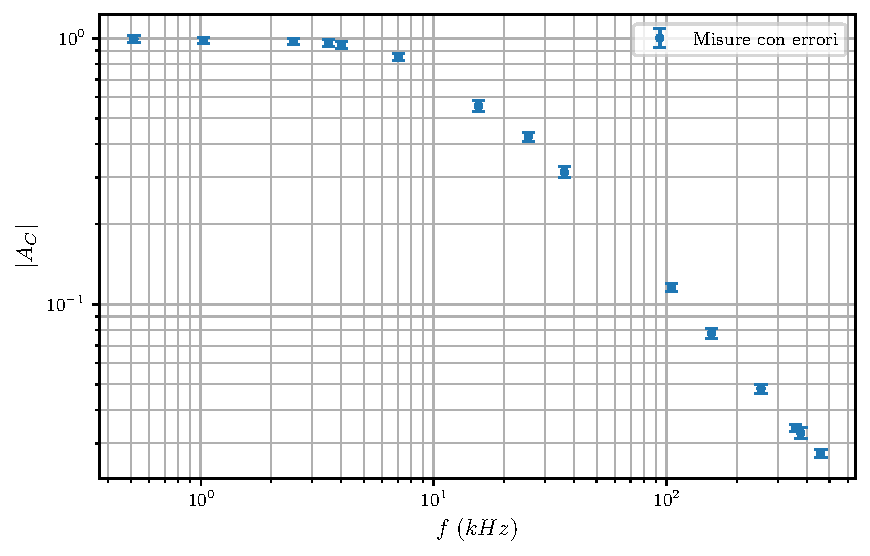
\includegraphics{onda_sin_AC(f).pdf}
    \caption{Grafico logaritmico di $|A_{C}|(f)$}
    \label{fig:funzione di trasferimento C}
\end{figure}

È noto che la funzione di trasferimento in scala logaritmica assuma un andamento lineare a frequenze elevate; è possibile quindi tracciare una retta di pendenza $-1$ passante per i punti situati all'estrema destra del grafico. Questa retta interseca l'asintoto orizzontale $|A_{C}| = 1$ alla frequenza di taglio $f_{0}$.

\begin{figure}[ht!]
    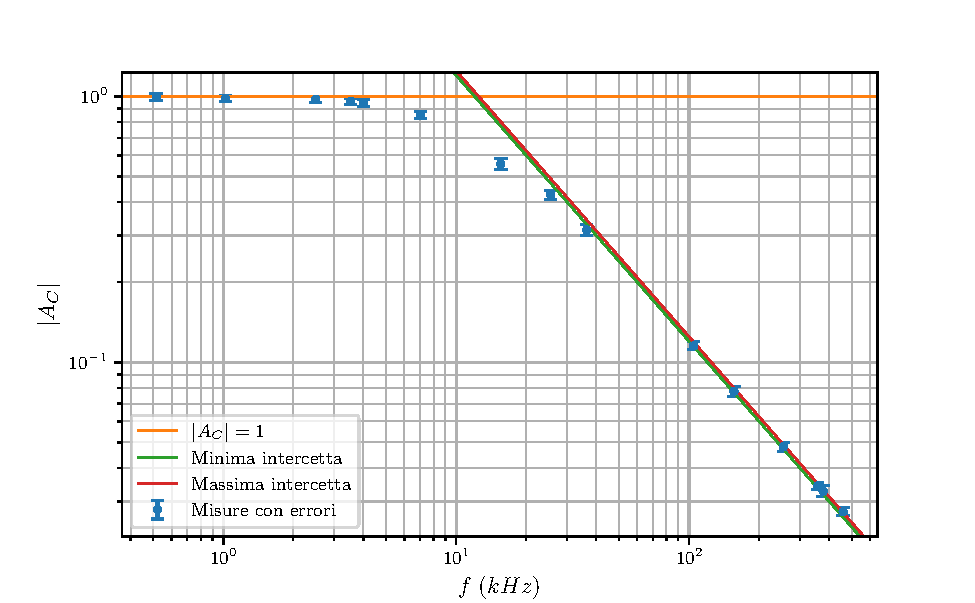
\includegraphics{onda_sin_AC(f)_taglio.pdf}
    \caption{Grafico della stima della frequenza di taglio}
    \label{fig:frequenza di taglio C}
\end{figure}

Uno zoom sull'intersezione delle rette è riportato in \autoref{fig:frequenza di taglio C zoom}%, mentre in \autoref{fig:frequenza di taglio C intercette} uno zoom sulle rette di massima e minima intercetta.

\begin{figure}[ht!]
    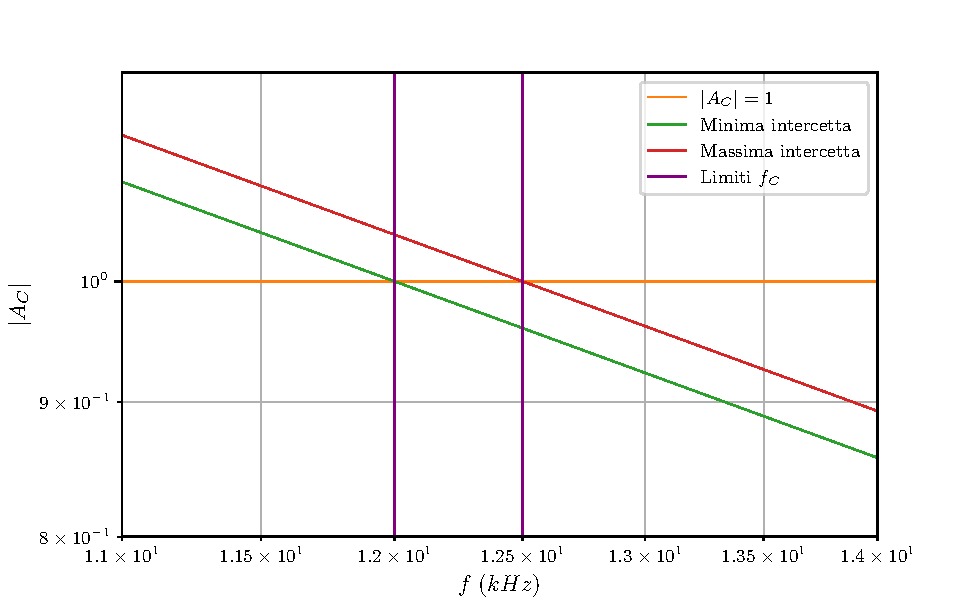
\includegraphics{onda_sin_AC(f)_taglio_frequenza.pdf}
    \caption{Zoom intersezione rette}
    \label{fig:frequenza di taglio C zoom}
\end{figure}

% \begin{figure}[ht!]
%     \centering
%     \begin{subfigure}[b]{0.44\textwidth}
%         % \import{../assets/}{circuito_osc_R.pdf_tex}
%         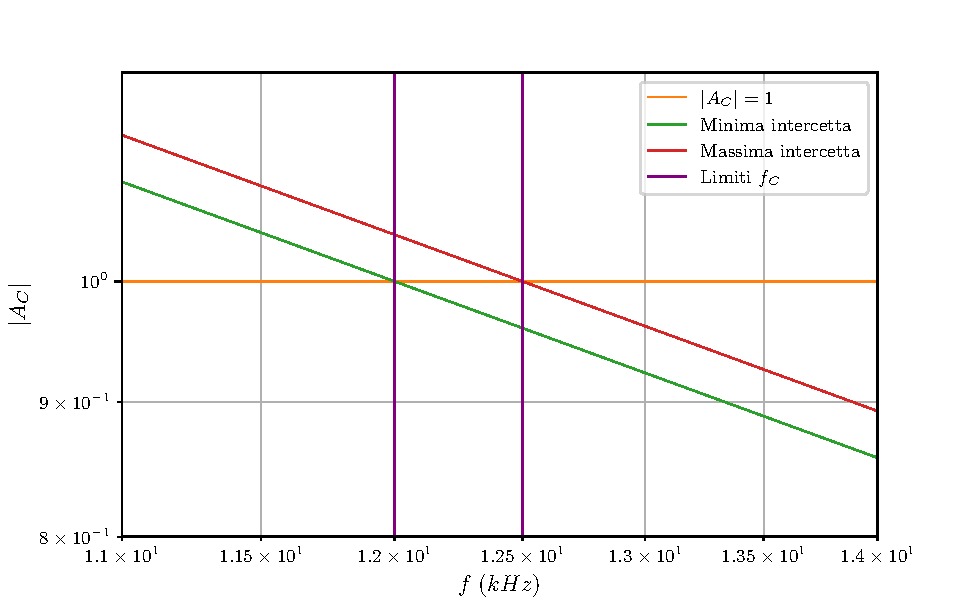
\includegraphics{onda_sin_AC(f)_taglio_frequenza.pdf}
%         \caption{Zoom intersezione rette}
%         \label{fig:frequenza di taglio C zoom}
%     \end{subfigure}
%     \hspace{0.1\textwidth}
%     \begin{subfigure}[b]{0.44\textwidth}
%         % \import{../assets/}{circuito_osc_C.pdf_tex}
%         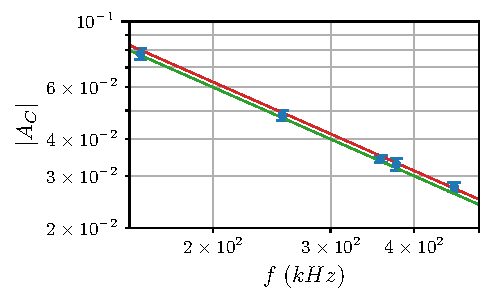
\includegraphics{onda_sin_AC(f)_taglio_intercette.pdf}
%         \caption{Zoom massima e minima intercetta}
%         \label{fig:frequenza di taglio C intercette}
%     \end{subfigure}
%     \caption{Zoom \autoref{fig:frequenza di taglio C}}
%   \end{figure}

\begin{align*}
    f_{0 \; min} &= 12.0 \; kHz \\
    f_{0 \; max} &= 12.5 \; kHz
\end{align*}

\begin{align*}
    f_{0 \; best} &= \frac{f_{0 \; max} + f_{0 \; min}}{2} = 12.25 \approx 12.3 \; kHz \\
    \delta f_{0} &= \frac{f_{0 \; max} - f_{0 \; min}}{2} = 0.25 \approx 0.3 \; kHz
\end{align*}

Quindi il valore di \(f_{0} = (12.3 \pm 0.3) \; kHz\).

%sezione phi
\hline

%
%plot fase
%

Non avendo potuto raccogliere dati sufficientemente vicini ad $f_{0}$, non è possibile evidenziare chiaramente la regione di linearità. %check readme

%Abbiamo quindi tracciato le rette di massima e minima intercetta passanti per i punti $(f_{0} - \delta f_{0}, -\pi/4)$ e $(f_{0} + \delta f_{0}, -\pi/4)$ in modo da poter osservare come il punto $(15.55, -0.90)$ è sufficientemente vicino alla frequenza di taglio da intersecare le rette con le sue barre d'errore.

% Per trovare la pendenza delle rette da tracciare, abbiamo valutato la derivata di (...)

\newpage

\subsection{Funzione di trasferimento ai capi di $R$}

Con i dati raccolti si calcola il modulo della funzione di trasferimento $|A_{R}|$ al variare della frequenza utilizzando l' %cosa

\subsubsection{Dati ed errori}

% \begin{table}[ht!]
%     \centering
%     \caption{Misure dell'onda sinusoidale ai capi di $R$}
%     \import{../tables/}{onda_sin_VR.tex}
%     \label{tab:misure onda sinusoidale R}
% \end{table}

% todo: tabella misure ai capi di R

\subsubsection{Analisi dati}

% todo: grafico con caption: Grafico logaritmico di $|A_{R}|(f)$

\section{Conclusioni}

%qualcosa sulle funzioni di trasferimento ottenute?
%valore ottenuto sulla freq. di cutoff, eventuali considerazioni nel caso la si confronti con il t. di risposta del circuito
%c'è qualcosa che si può dire dei filtri passa-basso/alto? altrimenti togli questa riga

\end{document}
